\documentclass{article}%
\usepackage[T1]{fontenc}%
\usepackage[utf8]{inputenc}%
\usepackage{lmodern}%
\usepackage{textcomp}%
\usepackage{lastpage}%
\usepackage[head=40pt,margin=0.5in,bottom=0.6in]{geometry}%
\usepackage{graphicx}%
%
\title{\textbf{Habitantes de Maracaibo protestan por tener más de 24 horas sin luz}}%
\author{El Nacional Web}%
\date{17/09/2018}%
%
\begin{document}%
\normalsize%
\maketitle%
\textbf{URL: }%
http://www.el{-}nacional.com/noticias/sociedad/habitantes{-}maracaibo{-}protestan{-}por{-}tener{-}mas{-}horas{-}sin{-}luz\_252032\newline%
%
\textbf{Periodico: }%
EN, %
ID: %
252032, %
Seccion: %
Sociedad\newline%
%
\textbf{Palabras Claves: }%
Luz, Zulia\newline%
%
\textbf{Derecho: }%
2.8, %
Otros Derechos: %
, %
Sub Derechos: %
2.8.1\newline%
%
\textbf{EP: }%
SI\newline%
\newline%
%
\textbf{\textit{El apagón podría estar afectando a más de 60\% de la población en el estado zuliano~}}%
\newline%
\newline%
%
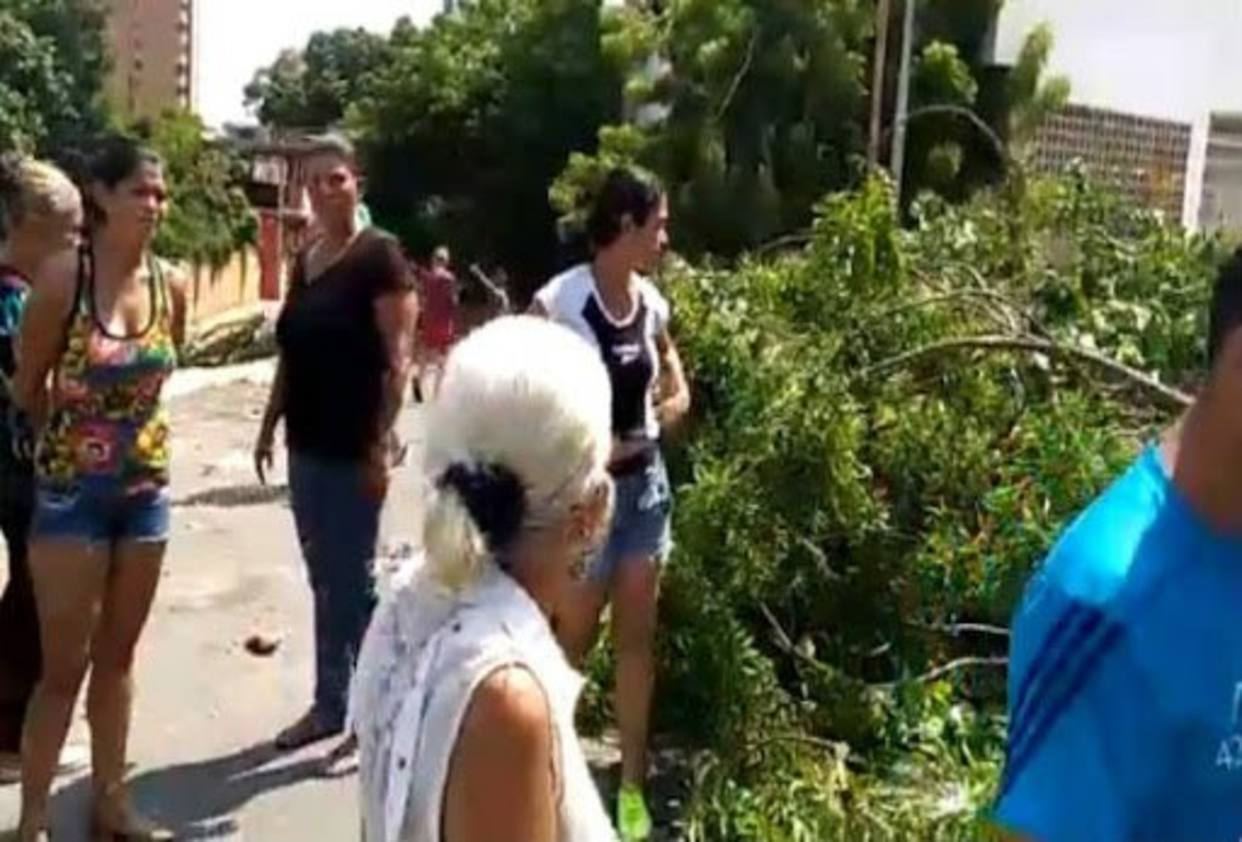
\includegraphics[width=300px]{214.jpg}%
\newline%
%
Este lunes, un grupo de vecinos en Maracaibo, estado Zulia, mantienen cerrado el paso en el sector La Virginia~luego de estar más de 24 horas sin servicio eléctrico.%
\newline%
%
Jesús Murillo, habitante de la zona, afirmó que los ciudadanos no han dormido desde hace un día por la falta del servicio, por~lo que decidieron salir a protestar ante la falta de respuesta de los entes correspondientes.%
\newline%
%
Algunos sectores afectados con la falla son Primero de Mayo, Nueva Vía, San Jose, La Limpia, Santa Maria, La Paragua, El Portón, Calles 72, Tierra Negra, Delicias, Bella Vista, Terrazas de Lago y La Pomona.%
\newline%
%
Reportes informan que estos sitios poseen más de cinco horas sin luz, lo que representa un 60\%~de Maracaibo sin energía eléctrica, de acuerdo a la información del periodista Gerard Torres.%
\newline%
%
\end{document}